% !TEX program = lualatex
% !BIB program = bibtex
\documentclass[8pt,dvipsnames,table]{beamer}

% ==============================================================================
% Language and Encoding
% ==============================================================================
\usepackage[utf8]{inputenc}
\usepackage[english]{babel}
\usepackage[square,sort]{natbib}

% ==============================================================================
% Font
% ==============================================================================
% \usefonttheme{professionalfonts}
% \usefonttheme{serif}
% \usepackage{fontspec}
% \setmainfont{Helvetica Neue}
\usepackage{helvet}
\usepackage{lmodern}

% ==============================================================================
% Color, style and layout
% ==============================================================================
\usepackage{xcolor}
\usepackage{graphicx}
\usepackage{hyperref}
\usepackage{bm}
\usepackage{subfig}
\usepackage{pict2e}
\usepackage{comment}
\usepackage{pdfpages}
\usepackage{geometry}
% \usepackage[paper=landscape]{typearea}

% ==============================================================================
% Math and Physics
% ==============================================================================
\usepackage{mathrsfs}
\usepackage{physics}
\usepackage{slashed}
\usepackage{siunitx}
\usepackage{tikz-feynman}

% ==============================================================================
% Beamer backup
% ==============================================================================
\usepackage{appendixnumberbeamer}

% ==============================================================================
% Theme
% ==============================================================================
\usetheme{metropolis}
% \usecolortheme[snowy]{owl}
\linespread{1.5}

% ==============================================================================
% Macros
% ==============================================================================
%\newcommand{\phanitem}{\phantom{\item}}
\newcommand{\lag}{\mathcal{L}}
\newcommand{\Mcal}{\mathcal{M}}
\newcommand{\g}{\gamma}
\renewcommand{\a}{\alpha}
\newcommand{\s}{\sigma}

% ==============================================================================
% Color Command
% ==============================================================================
% \definecolor{red}{rgb}{1, 0., 0.}

\newcommand{\red}[1]{{\color{OrangeRed}#1}}
\newcommand{\orange}[1]{{\color{Bittersweet}#1}}
\newcommand{\blue}[1]{{\color{NavyBlue}#1}}
\newcommand{\green}[1]{{\color{ForestGreen}#1}}
\newcommand{\purple}[1]{{\color{RedViolet}#1}}

% ==============================================================================
% Itemize style
% ==============================================================================
\setbeamertemplate{itemize item}{$\square$}

% ==============================================================================
% Horizontal Alignment
% ==============================================================================
\makeatletter
\newcommand{\pushright}[1]{\ifmeasuring@#1\else\omit\hfill$\displaystyle#1$\fi\ignorespaces}
\newcommand{\pushleft}[1]{\ifmeasuring@#1\else\omit$\displaystyle#1$\hfill\fi\ignorespaces}
\makeatother

% ==============================================================================
% Graphics Path
% ==============================================================================
\graphicspath{./}

% ==============================================================================
% Title Page
% ==============================================================================
\title{Coulomb Resummation Near $t\bar t$ Threshold}
\author[Y. Huang]{Yingsheng Huang}
\institute[IHEP]{Institute of High Energy Physics}
\date



\begin{document}

\begin{frame}{}
	\maketitle
	% \par\medskip
	% \uncover<4->{\vsapce*{-3in}arxiv:1809.09023}
\end{frame}

\begin{frame}
	\frametitle{Outlines}
	\tableofcontents
\end{frame}

\begin{frame}
	\frametitle{The Idea}

	
	\begin{itemize}
		\item For a process near the threshold of a specific fermion (i.e. $s\sim(2m_f)^2$), the exchange of Coulomb mode gluon is important, and for each order of the perturbative expansion, this part contributes an amount of approximately the same order. 
		\item Perturbative expansion breaks down, resummation needed. 
		\item To resum all Coulomb gluon exchange diagrams, one can use pNRQCD and convert the problem to a differential equation problem. 
	\end{itemize}



\end{frame}

\section{\citet{Fadin1987}}
\begin{frame}
	\frametitle{\citet{Fadin1987}}

	Coulomb resummation for top pair production in the threshold region can be traced back to '87\citep{Fadin1987}.
	\begin{figure}[!htb]
		\centering
		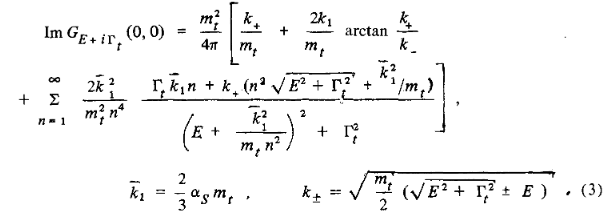
\includegraphics[width=\linewidth]{image1.png}
		% \caption{}
		\label{fig:image1}
	\end{figure}
	They discussed the total cross section of $e^+e^-\to t\bar t$ and the significance of this Coulomb effect at threshold varied with top mass (it was before the measurement of top mass in the '90s).

	\pause
	The details of their calculation should be in \textbf{\textit{Sov.J.Nucl.Phys. 48 (1988) 309-313}} which is nowhere to be found. \textbf{\textit{\citet{Strassler:1990nw}}} also gave a detailed description about $e^+e^-\to t\bar t$. 


\end{frame}

\section{\citet{Melnikov:1994jb}}
\begin{frame}
	\frametitle{\citet{Melnikov:1994jb}}

	They were mostly considering a pseudoscalar Higgs $A\to \gamma\gamma$ process in the context of MSSM, near $t\bar t$ threshold ($m_A=2m_t+E$, $E\ll m_A$).
	\begin{figure}[!htb]
		\centering
		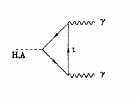
\includegraphics[]{image2.png}
		% \caption{}
		\label{fig:image2}
	\end{figure}
	There're also $W$ loops in $H\to \gamma\gamma$.

\end{frame}

\begin{frame}
	\frametitle{\citet{Melnikov:1994jb}}

	The diagrams are
	\begin{figure}[!htb]
		\centering
		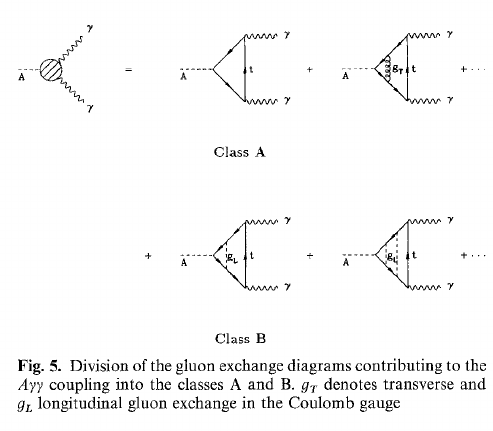
\includegraphics[width=0.8\linewidth]{image4.png}
		% \caption{}
		\label{fig:image4}
	\end{figure}


\end{frame}

\begin{frame}
	\frametitle{\citet{Melnikov:1994jb}}


	The $A\to\gamma\gamma$ amplitude is expressed as
	\begin{figure}[!htb]
		\centering
		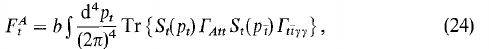
\includegraphics[width=0.8\linewidth]{image3.png}
		% \caption{}
		\label{fig:image3}
	\end{figure}\vspace{-0.1in}
	\only<1>{
		\begin{figure}[!htb]
			\centering
			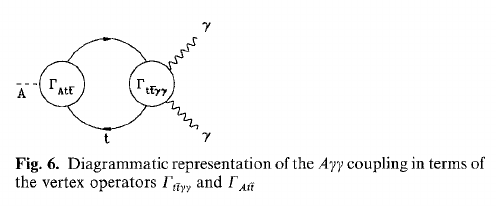
\includegraphics[width=0.8\linewidth]{image5.png}
			% \caption{}
			\label{fig:image5}
		\end{figure}
		The top propagator with width is
		\begin{figure}[!htb]
			\centering
			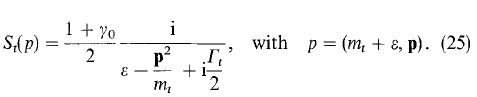
\includegraphics[width=0.8\linewidth]{image6.png}
			% \caption{}
			\label{fig:image6}
		\end{figure}
	}
	\only<2>{
		Take the leading order of $\Gamma_{At\bar t}$ which is just a coupling, and take $\Gamma_{t\bar t \gamma\gamma}$ to include all Coulomb gluon exchanges.
		\begin{figure}[!htb]
			\centering
			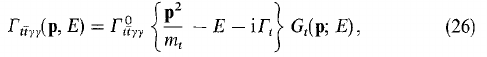
\includegraphics[width=0.8\linewidth]{image7.png}
			% \caption{}
			\label{fig:image7}
		\end{figure}
		$\Gamma_{t\bar t \gamma\gamma}^0$ is also the coupling of $t\bar t\to \gamma\gamma$.
	}



\end{frame}

\begin{frame}
	\frametitle{\citet{Melnikov:1994jb}}

	Solve the Schr\"odinger equation
	\begin{figure}[!htb]
		\centering
		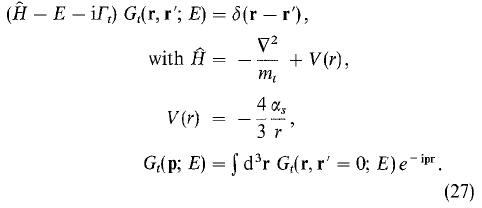
\includegraphics[width=0.8\linewidth]{image8.png}
		% \caption{}
		\label{fig:image8}
	\end{figure}

\end{frame}

\begin{frame}
	\frametitle{\citet{Melnikov:1994jb}}


	\begin{figure}[!htb]
		\centering
		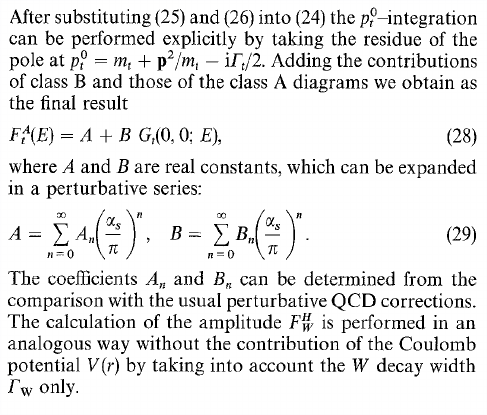
\includegraphics[width=.8\linewidth]{image15.png}
		% \caption{}
		\label{fig:image15}
	\end{figure}


\end{frame}

\begin{frame}
	\frametitle{}

	To do this matching they have some predetermined results
	\begin{figure}[!htb]
		\centering
		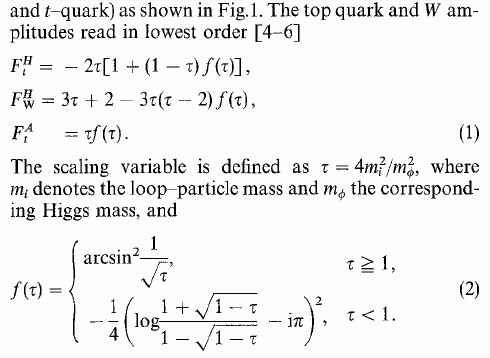
\includegraphics[width=.8\linewidth]{image16.png}
		% \caption{}
		\label{fig:image16}
	\end{figure}
	And by expanding $F_t^A$ near $\tau=1$, the value of $A_n$ and $B_n$ is obtained.

\end{frame}

\begin{frame}
	\frametitle{Result of $G$}

	The result of a stable top is
	\begin{figure}[!htb]
		\centering
		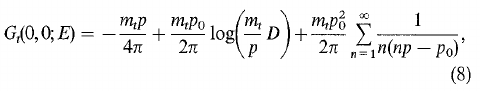
\includegraphics[width=.8\linewidth]{image11.png}
		% \caption{}
		\label{fig:image11}
	\end{figure}
	\begin{figure}[!htb]
		\centering
		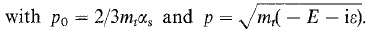
\includegraphics[width=.5\linewidth]{image12.png}
		% \caption{}
		\label{fig:image12}
	\end{figure}
	D is a real renormalization artifact.

	To get a result with finite width, one perform the substitution
	\begin{figure}[!htb]
		\centering
		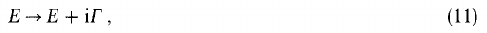
\includegraphics[width=.8\linewidth]{image13.png}
		% \caption{}
		\label{fig:image13}
	\end{figure}
	and
	\begin{figure}[!htb]
		\centering
		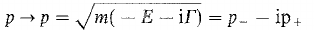
\includegraphics[width=.5\linewidth]{image14.png}
		% \caption{}
		\label{fig:image14}
	\end{figure}
	\begin{figure}[!htb]
		\centering
		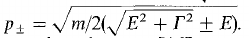
\includegraphics[width=.4\linewidth]{image10.png}
		% \caption{}
		\label{fig:image10}
	\end{figure}


\end{frame}

\begin{frame}
	\frametitle{Result of $G$}

	The result with finite top width is
	\begin{figure}[!htb]
		\centering
		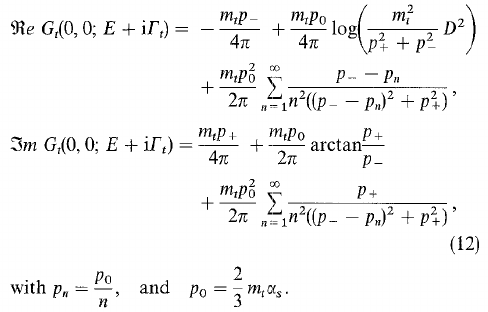
\includegraphics[width=.8\linewidth]{image9.png}
		% \caption{}
		\label{fig:image9}
	\end{figure}
	and
	\begin{figure}[!htb]
		\centering
		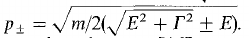
\includegraphics[width=.5\linewidth]{image10.png}
		% \caption{}
		\label{fig:image10}
	\end{figure}


\end{frame}

\begin{frame}
	\frametitle{Result of $G$}

	The summation in (8) is evaluated to be
	\begin{align}
		\sum_{i=1}^n\frac{1}{n(np-p_0)}=-\frac{\psi ^{(0)}\left(1-\frac{p_0}{p}\right)+\gamma_E }{p_0}=-\frac{H_{-p_{0}/p}}{p_0}
	\end{align}
	where $H_n\equiv\left(\sum_{i=1}^n1/i\right)$ is the harmonic number.

	In \citep{Bharucha:2016jyr} the summation isn't actually done to all order:
	\begin{figure}[!htb]
		\centering
		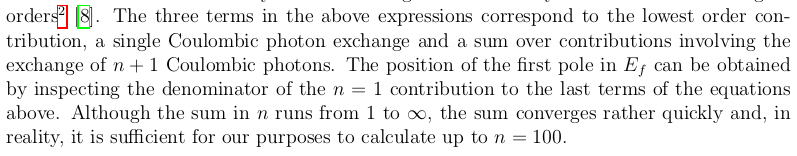
\includegraphics[width=\linewidth]{image40.png}
		% \caption{}
		\label{fig:image40}
	\end{figure}


\end{frame}

\begin{frame}
	\frametitle{Compare amplitudes}

	\only<1>{\begin{figure}[!htb]
		\centering
		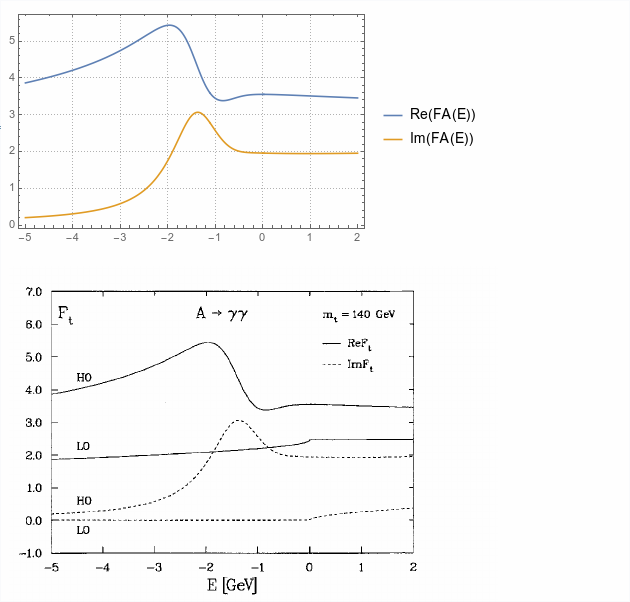
\includegraphics[width=.8\linewidth]{image42.png}
		% \caption{}
		\label{fig:image42}
	\end{figure}}
	
	

\end{frame}

\begin{frame}
	\frametitle{Shape of the Green function}

	\begin{figure}[!htb]
		\centering
		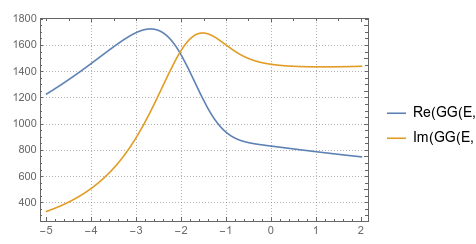
\includegraphics[width=\linewidth]{image43.png}
		% \caption{}
		\label{fig:image43}
	\end{figure}

\end{frame}

\begin{frame}
	\frametitle{Determine $A$, $B$}

	To determine the leading $A$ and $B$: Take $A\to\gamma\gamma$ as an example,
	\begin{align}
		G_t(E)=-\frac{m_t\sqrt{m_t(-E-i\epsilon)}}{4\pi}
	\end{align}
	And $F_t^A=\tau f(\tau)$ is expanded to be
	\begin{align}
		\frac{\pi ^2}{4}-i \pi  \sqrt{\tau -1}+\mathcal{O}(\tau-1)
	\end{align}
	The latter one, according to the definition of $\tau$ is expressed as
	\begin{align}
		- \pi  \sqrt{\frac{-E-i\epsilon}{m_t}}
	\end{align}
	which leads to the final result
	\begin{figure}[!htb]
		\centering
		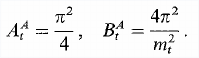
\includegraphics[width=.4\linewidth]{image17.png}
		% \caption{}
		\label{fig:image17}
	\end{figure}


\end{frame}

\begin{frame}
	\frametitle{Further QCD Corrections}

	\begin{figure}[!htb]
		\centering
		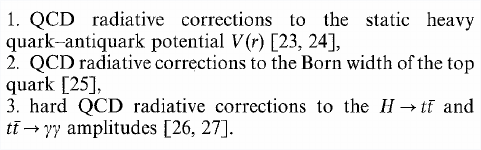
\includegraphics[width=.8\linewidth]{image18.png}
		% \caption{}
		\label{fig:image18}
	\end{figure}
	The 1st one is done by considering the running of $\alpha_s$.

	The 2nd one is not considered (too small).

	The 3rd one: see next page

\end{frame}
\begin{frame}
	\frametitle{Further QCD Corrections}

	\begin{figure}[!htb]
		\centering
		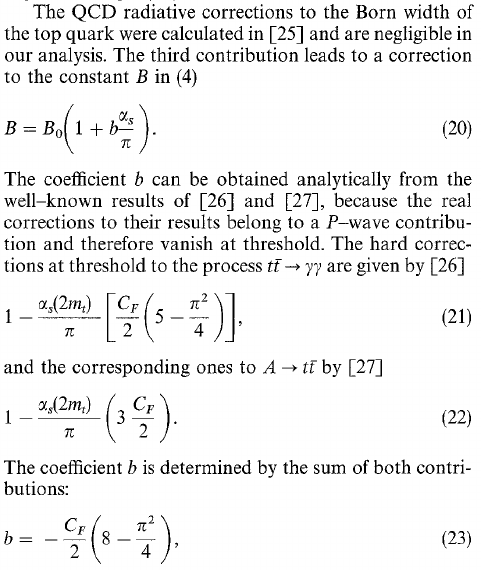
\includegraphics[width=.65\linewidth]{image19.png}
		% \caption{}
		\label{fig:image19}
	\end{figure}


\end{frame}

\section{\citet{Beneke:2013jia}}
\begin{frame}
	\frametitle{Diagrams}

	\begin{figure}[!htb]
		\centering
		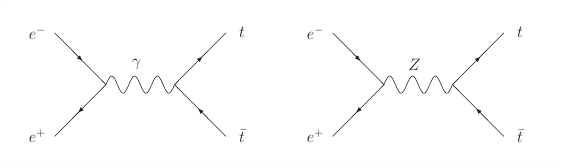
\includegraphics[width=\linewidth]{image20.png}
		% \caption{}
		\label{fig:image20}
	\end{figure}


\end{frame}
\begin{frame}
	\frametitle{Heavy quark current correlation function}

	\begin{figure}[!htb]
		\centering
		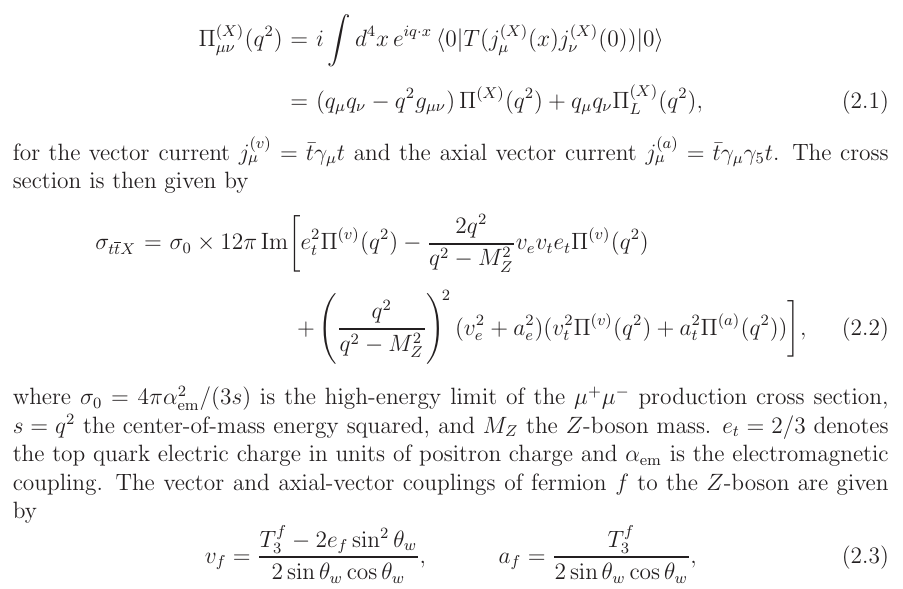
\includegraphics[width=\linewidth]{image21.png}
		% \caption{}
		\label{fig:image21}
	\end{figure}


\end{frame}
\begin{frame}
	\frametitle{Match to NRQCD}

	\begin{figure}[!htb]
		\centering
		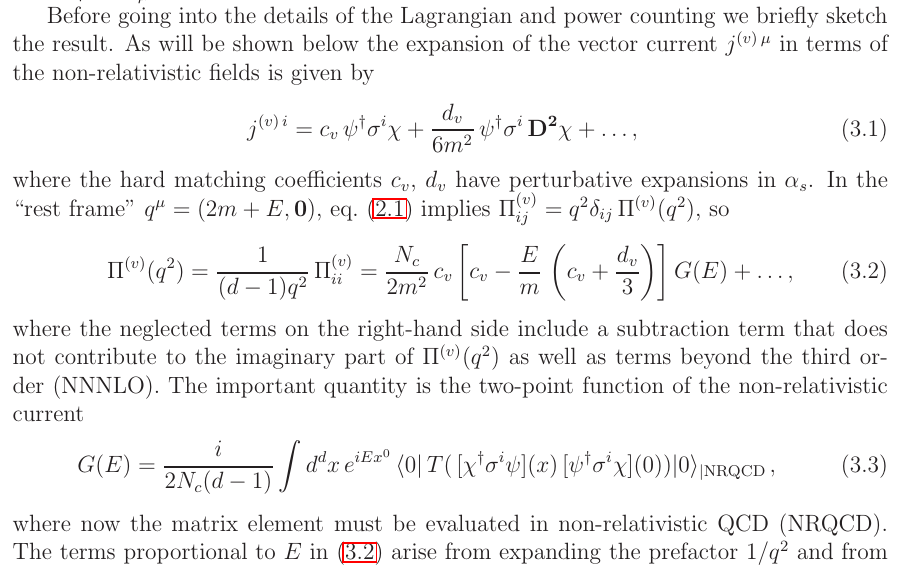
\includegraphics[width=\linewidth]{image22.png}
		% \caption{}
		\label{fig:image22}
	\end{figure}


\end{frame}

\begin{frame}
	\frametitle{Match to NRQCD}

	\begin{figure}[!htb]
		\centering
		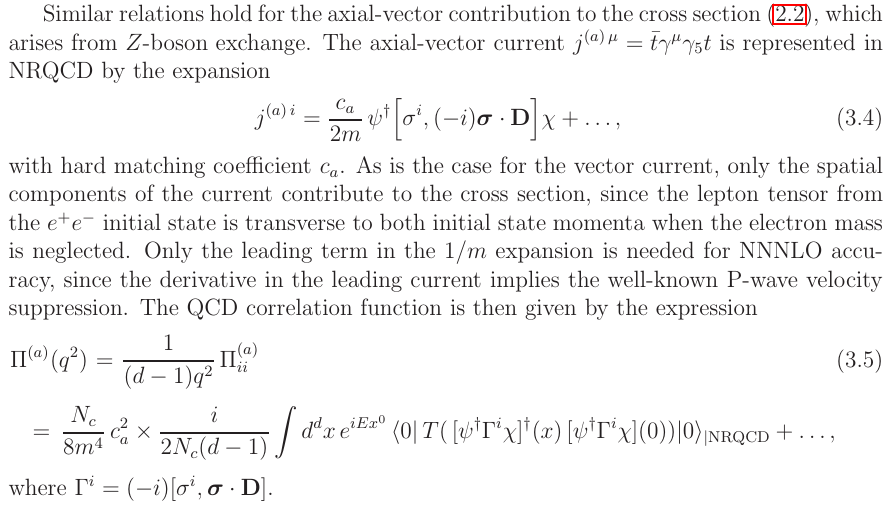
\includegraphics[width=\linewidth]{image23.png}
		% \caption{}
		\label{fig:image23}
	\end{figure}


\end{frame}

\begin{frame}
	\frametitle{Match to PNRQCD}

	\begin{figure}[!htb]
		\centering
		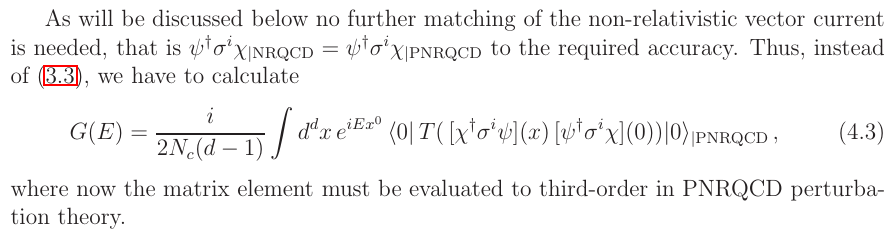
\includegraphics[width=\linewidth]{image24.png}
		% \caption{}
		\label{fig:image24}
	\end{figure}

	Lagrangian:
	\begin{figure}[!htb]
		\centering
		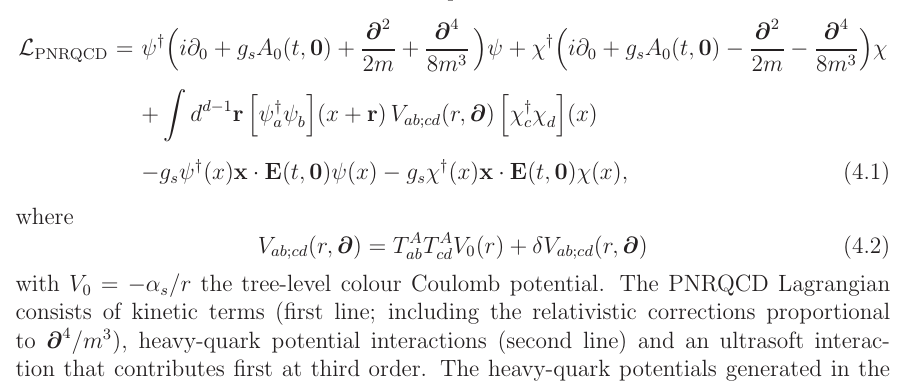
\includegraphics[width=\linewidth]{image25.png}
		% \caption{}
		\label{fig:image25}
	\end{figure}


\end{frame}

\begin{frame}
	\frametitle{Green function}

	The Lippmann-Schwinger equation for the leading order Green function $G_0$ is
	\begin{figure}[!htb]
		\centering
		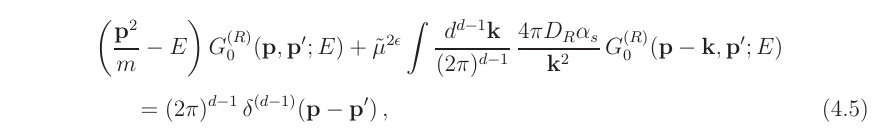
\includegraphics[width=\linewidth]{image26.png}
		% \caption{}
		\label{fig:image26}
	\end{figure}
	where R denotes color state, $D_1=-C_F$ and $D_8=-\left( C_F-C_A/2 \right)$.
	\begin{figure}[!htb]
		\centering
		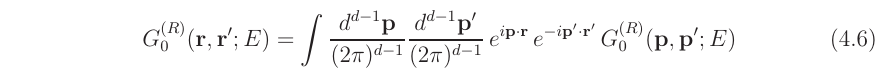
\includegraphics[width=\linewidth]{image27.png}
		% \caption{}
		\label{fig:image27}
	\end{figure}
	In 4-d the corresponding Schr\"odinger equation is
	\begin{figure}[!htb]
		\centering
		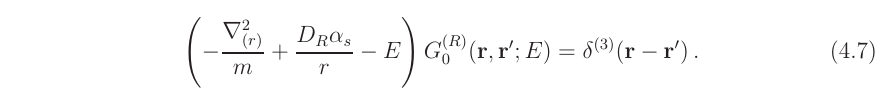
\includegraphics[width=\linewidth]{image28.png}
		% \caption{}
		\label{fig:image28}
	\end{figure}


\end{frame}

\begin{frame}
	\frametitle{Green function: Higher Order}

	\only<1>{
		\begin{figure}[!htb]
			\centering
			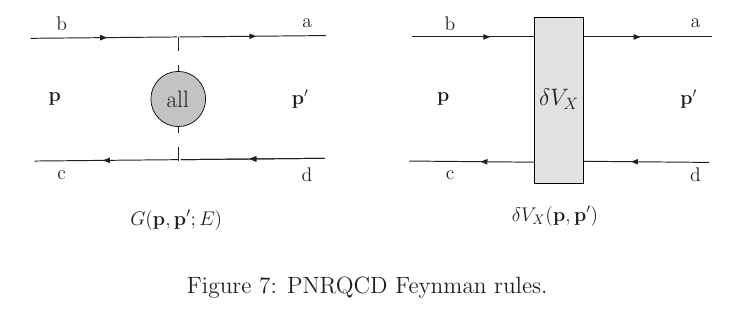
\includegraphics[width=.8\linewidth]{image30.png}
			% \caption{}
			\label{fig:image30}
		\end{figure}

		\begin{figure}[!htb]
			\centering
			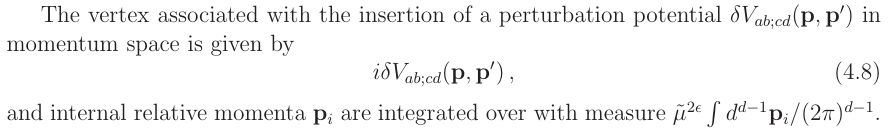
\includegraphics[width=\linewidth]{image29.png}
			% \caption{}
			\label{fig:image29}
		\end{figure}
		\begin{figure}[!htb]
			\centering
			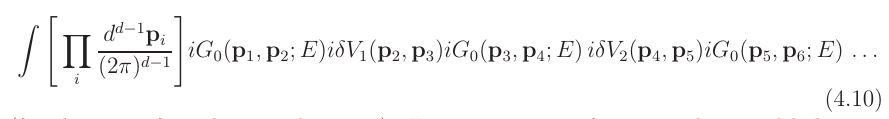
\includegraphics[width=\linewidth]{image31.png}
			% \caption{}
			\label{fig:image31}
		\end{figure}}
	\only<2>{
		For higher orders, some methods are discussed in \citep{Hoang:2000yr}:
		\begin{itemize}
			\item Hoang–Teubner	(HT), solved the NNLO Schr ̈odinger equation exactly in momentum space representation.
			\item Melnikov–Yelkhovsky–Yakovlev–Nagano–Ota–Sumino (MYYNOS), solved the NNLO Schr ̈odinger equation exactly in coordinate space representation. 
			\begin{figure}[!htb]
				\centering
				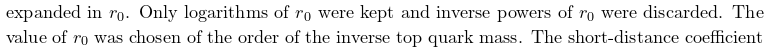
\includegraphics[width=\linewidth]{image41.png}
				% \caption{}
				\label{fig:image41}
			\end{figure}
			\item Penin--Pivovarov (PP), solved the NNLO Schr ̈odinger equation perturbatively in coordinate space representation. 
			\item Beneke–Signer–Smirnov (BSS), solved the NNLO Schr ̈odinger equation perturbatively using dim-reg. 
		\end{itemize}
	}

\end{frame}

\begin{frame}
	\frametitle{Derivation (Diagrams)}

	\only<1>{
		Consider the sum of all ladder diagrams:
		\begin{figure}[!htb]
			\centering
			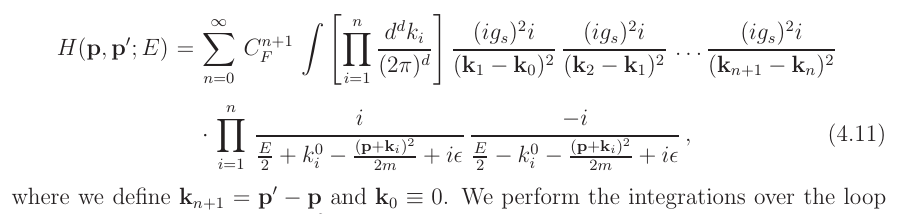
\includegraphics[width=\linewidth]{image32.png}
			% \caption{}
			\label{fig:image32}
		\end{figure}
		After integrated out $k^0$s
		\begin{figure}[!htb]
			\centering
			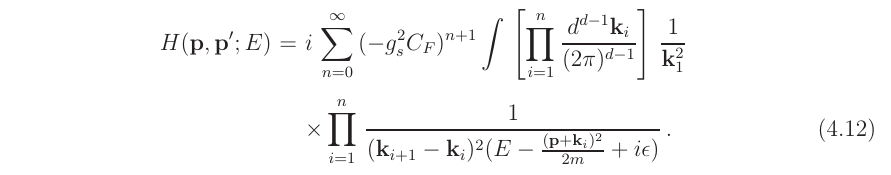
\includegraphics[width=\linewidth]{image33.png}
			% \caption{}
			\label{fig:image33}
		\end{figure}
	}
	\only<2>{
		\begin{figure}[!htb]
			\centering
			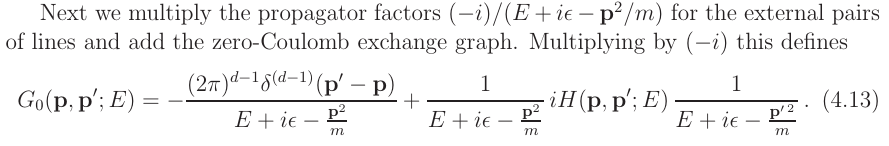
\includegraphics[width=\linewidth]{image34.png}
			% \caption{}
			\label{fig:image34}
		\end{figure}
		which satisfies the Lippmann-Schwinger equation for $G_0$. Higher orders
		\begin{figure}[!htb]
			\centering
			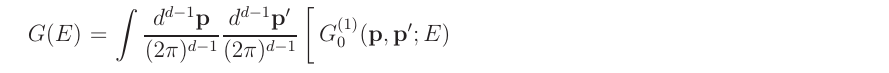
\includegraphics[width=\linewidth]{image35.png}\\
			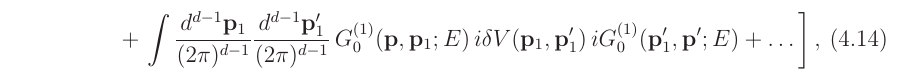
\includegraphics[width=\linewidth]{image36.png}
			% \caption{}
			\label{fig:image36}
		\end{figure}
		The spin indices is included
		\begin{figure}[!htb]
			\centering
			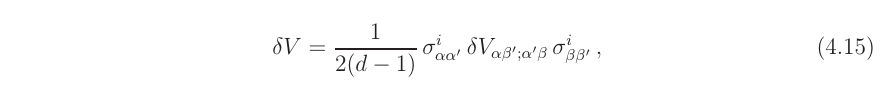
\includegraphics[width=\linewidth]{image37.png}
			% \caption{}
			\label{fig:image37}
		\end{figure}
		with normalization

	}


\end{frame}

\begin{frame}
	\frametitle{Explicit forms of the propagator (Coulomb Green function)
	}

	\only<1>{
		\begin{figure}[!htb]
			\centering
			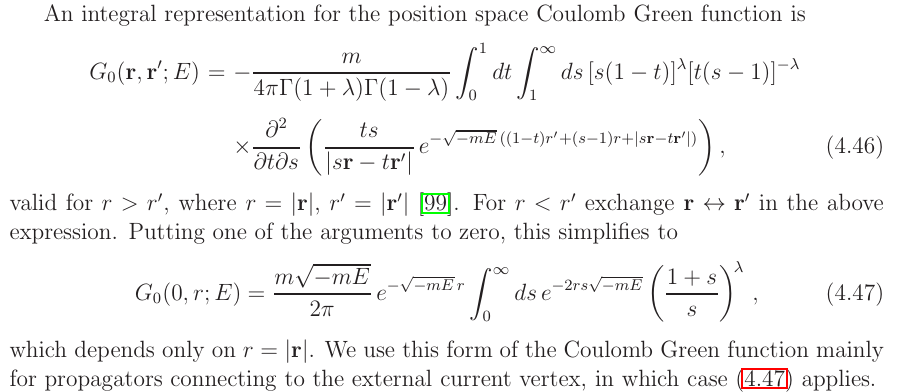
\includegraphics[width=\linewidth]{image38.png}
			% \caption{}
			\label{fig:image38}
		\end{figure}

	}
	\only<2>{
		\begin{figure}[!htb]
			\centering
			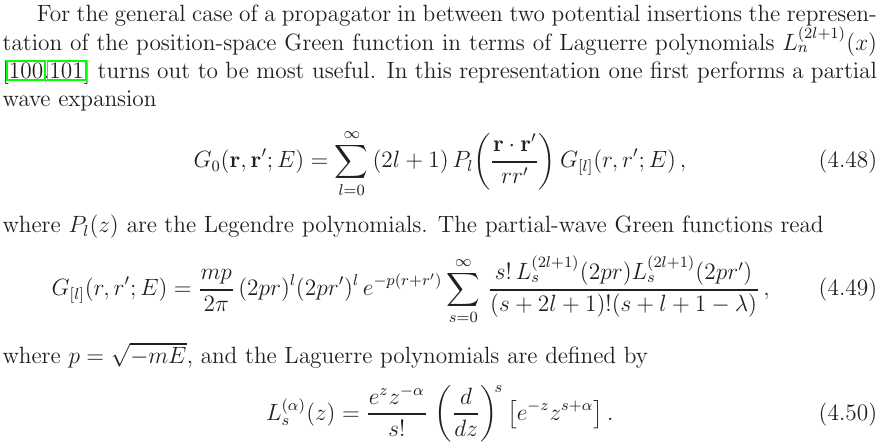
\includegraphics[width=\linewidth]{image39.png}
			% \caption{}
			\label{fig:image39}
		\end{figure}

	}

\end{frame}


\section*{END}
\begin{frame}[standout]
	\Huge Questions?
\end{frame}
% \begin{frame}
% 	\begin{center}
% 		\Huge 
% 		\usebeamercolor[bg]{frametitle}
% 		\emph{Thanks for your attention!}
% 	\end{center}
% \end{frame}

\appendix
\begin{frame}
	\vfill
	\centering
	\begin{beamercolorbox}[sep=8pt,center,shadow=true,rounded=true]{title}
		\usebeamerfont{title}Backup\par%
	\end{beamercolorbox}
	\vfill
\end{frame}

\bibliography{../Bib}
\bibliographystyle{apalike}

\end{document}